\section{Reporting and Publishing}
MSL staff report on activities in a number of ways. Of particular importance are the metrological reports (calibration and test reports) issued by MSL. These are covered in the next section (\S\ref{ss:metrological_reports}). 

A variety of other works may be produced for `publication' outside MSL, including:
\begin{itemize}
\item Scientific journal and conference papers (peer-reviewed or not)
\item Conference posters + presentation slides
\item Callaghan Innovation technical reports
\item Trade journal articles
\item International measurement comparison reports
\item Reports/submissions to technical committees (TCs, CCs, …)
\item MSL consultancy reports
\item MSL Technical Guides
\item MSL training course slides and notes
\item MSL software manuals (for external use)
\item Items for MSL web pages
\item Web-based videos (YouTube channel)   
\item MSL newsletter
\item Publicity material
\end{itemize}

Section~\ref{ss:msl_publications_policy} describes MSL policy for this broader category of publication.

Measurement results shall be traceable to primary measurement standards held by MSL, or other NMIs. A statement to this effect is included on all calibration and test report covers(~see  \cite[\S\ref*{GRP-ss:report_covers}]{MSL_Reporting_Guidelines}~). Any exceptions to this policy must be approved by the Chief Metrologist (~see~\S\ref{ss:msl_publications_policy}~).

\subsection{Metrological Reports}
\label{ss:metrological_reports}
Metrological reports are of high importance to MSL, so an elaborate system has been developed to ensure that they are of consistently high quality.

\subsubsection{Report types}
A metrological report will be one of the following types:
\begin{itemize}
\item Calibration Report - entitled ``Report on the Calibration of \ldots" or ``Report on the Measurement of \ldots'' 

A Calibration Report is used for IANZ classes beginning ``5'', except when the instrument or device under test is deemed to be unfit for calibration (in which case the measurement results may be issued in a ``Report on the Failure of \ldots'').

\item Test Report - entitled "Report on the Test of \ldots''  

A Test Report may be used for IANZ classes beginning ``5" or ``6"
\end{itemize} 

\subsubsection{Authority to write and review reports}
A person designated as a `worker' will carry out calibration or test work and write the report; a person designated as a 'checker' will check the measurements and the report. The worker(s) and checker share responsibility for the report.

The last page in the body of the report shall be signed, and all other pages initialled, by the worker, the checker, and the Chief Metrologist (or delegate). 

For IANZ-endorsed reports, either the worker or checker signing the report must be an IANZ signatory for the measurement class(es) covering the measurements.

The report shall be reviewed by the checker with respect to the following: 
\begin{itemize}
\item there is sufficient documentary evidence of the measurements made;
\item the process used is described in a technical procedure, or procedures, and that each procedure used has a current validation and has been correctly interpreted (where `current validation' is understood to mean that the technical procedure is valid on the report date);

Note, see \S\ref{sss:technical_procedure_structure} for validity requirements when a supporting procedure provides part of a traceability chain.

\item records clearly show who did the checking and what was checked (for routine work a checklist is recommended).
\end{itemize} 

The report must be reviewed by the Chief Metrologist, or delegate, to ensure that:
\begin{itemize}
\item the report has been written and checked as required above;
\item the report is free of typographical errors or inconsistencies;
\item the correct front cover has been used, indicating whether the measurements are within the IANZ scope of accredited services and whether the measurements are within MSL's CMCs (see also \S\ref{sss:measurement_conditions} regarding measurement conditions);
\item for IANZ-endorsed reports, at least one signatory has been approved;
\item the report date should normally be less than one month before the date that the report is signed.
\end{itemize} 

\subsubsection{Reporting measurement conditions}
\label{sss:measurement_conditions}
Sometimes, conditions of measurement are reported that involve quantities from a different technical discipline. For example, when calibrating a thermometry resistance bridge, staff with specialist knowledge in temperature measurement report a value of sensing current (an electrical quantity). Staff qualified to carry out the technical procedure (i.e., who appear in the Technical Competency Matrix for that procedure) are considered to have the expertise to assess associated measurement conditions. This is confirmed by external peer-review of signatories by IANZ. Therefore, reporting of measurement conditions is assumed to be compatible with the MSL scope of accreditation and the signatory status of the staff involved.

\subsubsection{Reporting format}
Details about the reporting format requirements are given in the Metrological Reports section of the MSL Guidelines on Reporting and Publishing \cite[\S\ref*{GRP-s:metrological_reports}]{MSL_Reporting_Guidelines}.

\paragraph{Statement about applicability of results}
For most calibration work, the MSL report format clearly identifies the item(s) being calibrated or tested. However, there are some situations where MSL is effectively sent an item or items that may be considered, from the point of view of the client, as a sample from a larger population (e.g., a piece of shade-cloth sent to MSL for characterisation). In all such cases, the MSL report shall clearly state that the results provided relate only to the item(s) actually measured. This is a requirement of the 17025:2018 standard \cite[clause 7.8.2.1~(l)]{ISO_17025}.      

\subsubsection{Issuing Paper Reports and Summary Data}

Only one printed report shall be signed and sent to the client. 

A scanned copy of this signed report shall be filed in the central file system ( see~\S\ref{ss:central_file_system} ). 

An electronic copy of the document used to create the report shall be retained in the section file system ( see~\S\ref{ss:section_file_systems} ). 
   
The client may be supplied with a copy of the scanned PDF version of the signed report, if requested.

A laminated card of the table of corrections may be supplied to the client, if required.  This card will show: the name of the instrument, the serial number of the instrument, the MSL report number and the correction table data.  The card will go through the same checking process as described above.

Clients may request calibration information in electronic format, such as an Excel spreadsheet. Such information may be provided, but only after the report has been issued. The electronic data must be checked with the same care given to written reports. Moreover, it should be made clear to the client that the written report remains the authoritative document. 

Every effort should be made to ensure that the items calibrated or tested will be returned to the client at the same time as the report. If the report is delayed, the client should be informed. If it is known in advance that the report will be issued after return of the client's items, the client should be advised before the work begins.


\subsubsection{Issuing Electronic Reports and Summary Data}
\label{sss:issuing_electronic_reports}
\begin{itemize}

\item Ensure that a report in electronic format is acceptable to the client.

\item The electronic report file shall be signed (~see procedure in \S\ref{sss:electronic_signatures}~) and a record of this signing process shall be saved in the central file system (~see~\S\ref{ss:central_file_system}~). 

\item Sufficient information about the data and documents used to create the report shall be retained in the section file system to allow the report to be recreated (~see~\S\ref{ss:section_file_systems}~). 
   
\item The client will be supplied with a copy of the electronic report and the MD5 checksum for the file (~see ``Checking the integrity of a report file'', in \cite[\S\ref*{GRP-ss:file_integrity_md5}]{MSL_Reporting_Guidelines}~).

\item The following message should be provided to the client with the report (make appropriate replacements for \textit{<report ID>} and  \textit{<checksum>}):
\begin{quote}
MSL's electronic calibration, test and measurement reports are produced in the same format as paper reports, but are provided as electronic files (PDF format). Distributing electronic reports carries with it a small risk that the file may become corrupted, or inadvertently changed somehow, after it has left MSL. To address this, we provide what is called an MD5 checksum, which allows the integrity of a file to be checked. You can use the MD5 checksum to make sure that the file you receive is valid. MSL Technical Guide 43 explains how to do this (online: \url{https://www.measurement.govt.nz/download/55}).

\vspace{\baselineskip}
The MD5 checksum for report \textit{<report ID>} is:   \textit{<checksum>} 
\end{quote}

\item Clients may request other calibration information in electronic format, such as an Excel spreadsheet. Such information may be provided, but only after the report has been issued. The electronic data provided must be checked with the same care given to written reports. Moreover, it should be made clear to the client that the report remains the authoritative document. 

\end{itemize}


Every effort should be made to ensure that the items calibrated or tested will be returned to the client at the same time as the report. If the report is delayed, the client should be informed. If it is known in advance that the report will be issued after return of the client's items, the client should be advised before the work begins.

\subsubsection{Signing electronic reports}
\label{sss:electronic_signatures}
Technical information on how to produce a calibration report, with a suitable report cover and electronic signature images, is given in the ``Electronic reports''  section of \cite[\S\ref*{GRP-ss:electronic_reports}]{MSL_Reporting_Guidelines}.

The process required to create a record of signing for the quality system is as follows:

\begin{enumerate}
\item Create a PDF version of the report file
\item Upload the PDF file to the ``Calibration Reports'' library. Note, the file name should be in the following format:
\begin{quote}
\texttt{"section name"\_"section file number"\_year}
\end{quote}
\item Fill in the metadata for the report. For example,
\begin{center}
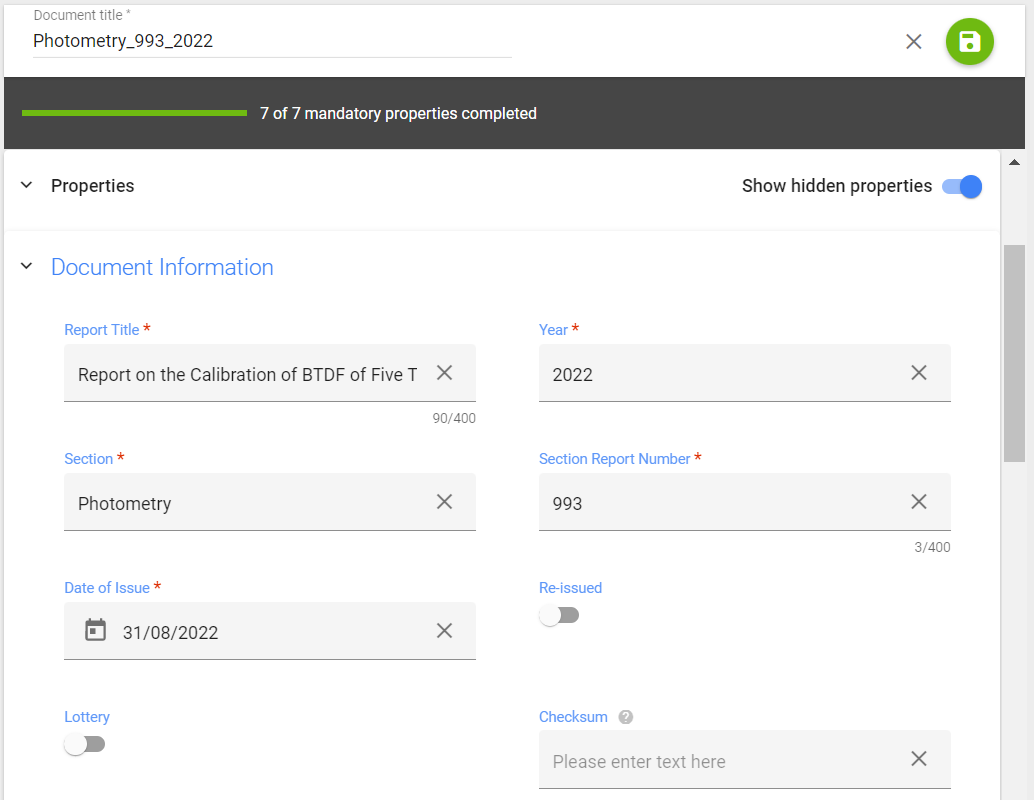
\includegraphics[scale=.9]{pictures/metadata_signed_report}
\end{center}
\item The first person can now `sign' the report by inserting an image of their signature using PDF reader software (~see \cite[\S\ref*{GRP-ss:electronic_reports}]{MSL_Reporting_Guidelines}~). The person who signed must upload the new version to EDI.

Note,
\begin{itemize}
\item the file name must not be changed (EDI maintains a version history based on file name)
\item it is not necessary to initial each page (as is done with paper reports)
\item for technical reasons, the document must be opened with a PDF reader running on a local machine (it is not possible to sign and re-store the document directly from a browser)
\end{itemize}

\item The second person can now `sign', following the process above.
\item Chief Metrologist, or delegate, can `sign'. 

Before uploading the final version, signed by everyone, an MD5 checksum must be calculated (~see \cite[\S\ref*{GRP-ss:file_integrity_md5}]{MSL_Reporting_Guidelines}~). 

During uploading of the final version, the MD5 checksum must be saved as a version `comment'. 

\item If corrections to the report are necessary during the signing process, the faulty version can be annotated with comments, highlighted sections, etc (using a PDF reader), and uploaded to EDI. Doing so maintains a full record of the signing/issuing process. 

Once corrected, the new report file must be signed again by everyone.
\end{enumerate}

This process generates a version history similar to the one below. All intermediate versions can be reviewed by clicking on the links at the left. Note the checksum in the comment associated with the final version.

\begin{center}
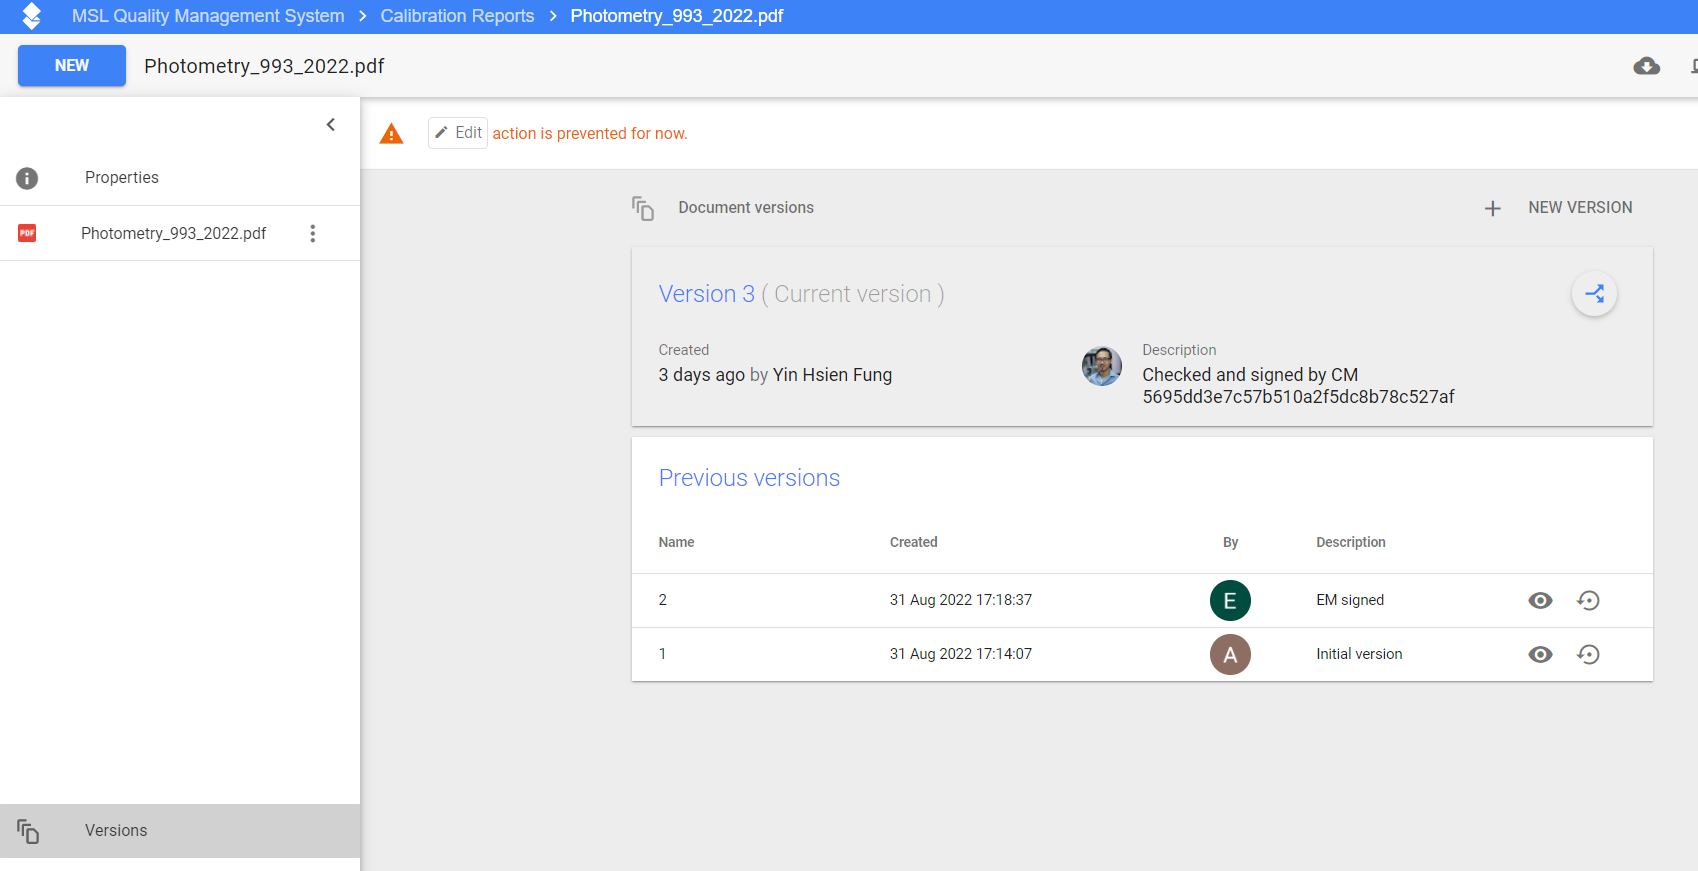
\includegraphics[scale=.6]{pictures/version_history_report}
\end{center}

\subsubsection{Withdrawal due to a reporting or measurement error}
\label{sss:reissue_report}
If any significant error is found in the most recent report on an instrument or artefact, within five years of first issue, the report must be withdrawn.``Significant'' would include a significant error of measurement or data processing, incorrect values, dates, serial numbers, etc, but not simple spelling or typing errors unless these could be misinterpreted.

In order to reissue the report, the instrument or artefact may need to be recalled so the test or calibration can be repeated. A new test date will be used if the test or calibration was repeated.

Any change of information in the reissued report shall be clearly identified and, where appropriate, the reason for change shall be given.

\paragraph{To withdraw paper reports}
\begin{enumerate}
\item Contact the client and ask for the return of the original report and also that any copies be destroyed. 

\item On receipt of the original report, stamp all pages ``{\color{red}CANCELLED}” and initial. 

\item Where paper photocopies are held by MSL, all pages should be stamped ``{\color{red}CANCELLED}” and initialled.

\item Electronic copies in the central file, and in the section file, should be cancelled:
\begin{itemize}
\item For a PDF file, add the text “{\color{red}CANCELLED}” to each page (in red text, with bold, large, font size – there are PDF reader programmes that can do this). 
\item For the central file copy, the name of the file should not be changed. Rather, the cancelled file should be saved with the same name and a note added about the cancellation in the EDI version history of the document. 
\end{itemize}

\item Produce a corrected report using the original report number.  Retain the original issue dates throughout, but add, after each issue date, the words `reissued on [new issue date]', e.g. `Report No. Pressure/1997/155, 11 August 1997, reissued on 10 February 2000'.

\item Any change of information in the report must be clearly identified and, where appropriate, the reason for the change should be included in the report (~some advice on formatting is given in \cite[\S\ref*{GRP-ss:reissued_reports}]{MSL_Reporting_Guidelines}~).

\item Reissue the corrected report and the cancelled original report to the client.

\item Make copies of the signed corrected original and file in the central file and the section file. 
\begin{itemize}
\item The name of the central file copy should not be changed (i.e., the new copy of the report replaces the cancelled original). 
\item A note should be added in the EDI version history to indicate a reissued report.
\item The metadata tag `reissued' for the EDI document should be set.
\end{itemize}

\end{enumerate}

\paragraph{To withdraw electronic reports}
\begin{enumerate}
\item Contact the client and ask that any copies be destroyed. 

\item Electronic copies in the central file, and in the section file, should be cancelled:
\begin{itemize}
\item For a PDF file, add the text “{\color{red}CANCELLED}” to each page (in red text, with bold, large, font size – there are PDF reader programmes that can do this). 
\item For the central file copy, the name of the file should not be changed. Rather, the cancelled file should be saved with the same name and a note added about the cancelation in the EDI version history of the document. 
\end{itemize}

\item Produce a corrected report using the original report number.  Retain the original issue dates throughout, but add, after each issue date, the words `reissued on [new issue date]', e.g. `Report No. Pressure/1997/155, 11 August 1997, reissued on 10 February 2000'.

\item Any change of information in the report must be clearly identified and, where appropriate, the reason for the change should be included in the report (~some advice on formatting is given in \cite[\S\ref*{GRP-ss:reissued_reports}]{MSL_Reporting_Guidelines}~).

\item Reissue the corrected report to the client with the new MD5 checksum. Send a copy of the cancelled original report to the client. 

\item File copies of the signed corrected original in the central file and the section file. 
\begin{itemize}
\item The name of the central file copy should not be changed (i.e., the new copy of the report replaces the cancelled original). 
\item Add a note to the EDI version history to indicate a reissued report.
\item Set the EDI document metadata tag `reissued'.
\end{itemize}
\end{enumerate}

\paragraph{Note} In general, changes to the central file should only be carried out by an MSL administrator or the Quality Manager. The procedure for signing electronic reports is an exception to this rule. 

\paragraph{Finally} If appropriate, amend the technical procedure associated with the report to reduce the likelihood of a similar mistake occurring in the future.

Also, if the likelihood of a similar error occurring in the future can be reduced by amending the Quality Manual, follow the Improvement Procedure.  




\subsubsection{Replacing a report at the client's request}
When a report has been lost, a replacement may be issued. 

\paragraph{Electronic reports} no special procedure is required to replace an electronic report. Simply dispatch a copy of the report to the client.

There is no need to record the replacement of the report in the central file system.


\paragraph{Paper reports}
The new report must be identified as a replacement and have a new report issue date (i.e. to ensure that any original is unique). The replacement must be signed and copies stored in the central file and section job file. 
\begin{itemize}
\item The first replacement of a lost report should be labelled ``Replacement of Report \ldots". 
\begin{itemize}
\item Retain the original issue dates throughout but add the words `reissued on (new issue date)', e.g.: ``Replacement of Report No. Pressure/1997/155, 11 August 1997, reissued on 10 February 2000".
\item Any subsequent replacements should be labelled ``Second Replacement of Report \ldots", etc.
\end{itemize}

\item Where an original signatory is not available, a person appointed to carry out the test and calibration work, or checking, in the designated field may sign the report per persona (p.p.).  The name of the original signatory must remain on the report.

\item Reissue the report to the client.

\item File copies of the report in the central file and the section file.
\begin{itemize}
\item The name of the central file copy should not be changed (i.e., the new copy of the report replaces the original). 
\item Add a note to indicate a replaced report in the EDI version history.
\item Set the EDI document metadata tag `reissued'.
\end{itemize}
\end{itemize}

Note, the client, on request, may be supplied with a copy of an original paper report, in which case the copy is not considered ``reissued". However, the client should be advised that the copy is not authoritative and, for example, may not be acceptable in court.

\subsubsection{Replacing a report issued with an incorrect report number}

A replacement may be issued if a report has been issued with an incorrect report number. 

Follow the first steps of the procedure in \S\ref{sss:reissue_report} for re-issuing a report, namely:

\begin{enumerate}
\item 
\begin{itemize} 
\item If a paper report was issued, contact the client and ask for the return of the original report and also that any copies be destroyed. 

\item If an electronic report was issued, ask the client to destroy all copies.
\end{itemize}

\item On receipt of an original paper report, stamp all pages ``{\color{red}CANCELLED}” and initial.

\item Where paper photocopies of paper reports are held by MSL, all pages should be stamped ``{\color{red}CANCELLED}” and initialled.

\item Electronic copies in the central file, and in the section file, should be cancelled:
\begin{itemize}
\item For a PDF file, add “{\color{red}CANCELLED}” to each page (in red text, with bold, large, font size – there are PDF reader programmes that can do this). 
\item Do not change the file name in the central file. Rather, the cancelled file should be saved with the same name and a note added to the EDI version history of the document about the cancellation. 
\end{itemize}
\end{enumerate}

The rest of the procedure is then as follows: 
\begin{enumerate}
\setcounter{enumi}{4}
\item The replacement report should use the correct (new) report number, followed by a line beginning ``Replacement of Report \ldots", which describes the previously issued report. For example, 
\begin{quote}
Report No.\ Humidity/2020/428, 3 March 2020\\
 Replacement of Report No.\ Humidity/2020/248, 16 February 2020
\end{quote}

\item The replacement report must be signed.
\begin{itemize}
\item Where an original signatory is not available, a person appointed to carry out the test and calibration work, or checking, in the designated field may sign the report per persona (p.p.).  The name of the original signatory must remain on the report.
\end{itemize}

\item Copies of the report must be stored in the central file and the section file.
\begin{itemize}
\item The name of the central file copy should be the new file name. (The old file name may be changed on EDI without breaking the version history. Seek help from the Quality Manager or site administrator to do this before uploading the new version of the file.) 
\item The central file metadata tag `reissued' should be set.
\item Add a note to the EDI version history to indicate a replaced report.
\end{itemize}
\item Reissue the report.

\end{enumerate}



\subsection{MSL Publications policy}
\label{ss:msl_publications_policy}

This section describes MSL policy for publications in general (other than the measurement reports described in \S\ref{ss:metrological_reports}). The policy is intended to enhance the science culture within MSL and mitigate risk to MSL's reputation by ensuring consistently high publication standards.   


It is intended that
\begin{itemize}
\item One of the MSL authors will take responsibility for coordinating the publication clearance process. 
%They should organise a reviewer and make sure that all relevant documents are stored in the repository. 

\item  Every document will be reviewed before publication, and some record of review will be kept. The potential for a publication to harm MSL's reputation shall be considered when deciding how to review a document. 

\item  Documents for publication will be made available to all MSL, usually by placing a copy in a common repository (~see~\S\ref{sss:publications_repository}~). A record of approvals will be kept with material in the repository 



\item  All measurement results reported shall be traceable to primary measurement standards held by MSL, or other NMIs (see notes below for exceptions)
%\end{itemize} 
%When this is not the case, a statement about the lack of traceability shall be included 
%\begin{itemize}
\item  No results will be published without the approval of the Chief Metrologist (or delegate) 
\end{itemize}

Notes: 
\begin{itemize}
\item Sometimes a publication may not seem sufficiently important to warrant a review. However, our experience has been that the review process is always beneficial.   
\item  The ease with which corrective action can be taken, if a problem is recognised after publication, may be taken into account when deciding how to review a document (e.g., it is easy to change material on the MSL website, but much harder to correct mistakes in an external publication). 
\item The review record  (in the repository) may briefly record that the work has been considered by someone to be of acceptable quality (a template for publication clearance is provided). Where appropriate, more detailed records of review can be kept.
%However, the review could also be detailed, or could contain information to locate details elsewhere (lab books, spreadsheet on the \deprecated{I-drive}~\proposed{G-drive}, etc).   
\item  Vigilance is needed to avoid unintentional publication of untraceable measurements. A notable example was the time-of-day widget displayed on the MSL website as `Official Time'.\footnote{Note, all traceable measurements will include an uncertainty statement and documentation that can be independently checked as evidence of traceability and accuracy.}
\item  Very rarely, untraceable measurements may be approved for publication by the Chief Metrologist. In such cases, a clear statement about the lack of traceability must accompany the results (see the section `Informal reporting of measurements' in the Guidelines on Reporting and Publishing \cite[\S\ref*{GRP-ss:informal_reporting}]{MSL_Reporting_Guidelines}). 

%\vspace{\baselineskip}
It may at the same time be possible to offer useful advice. For instance, 
\begin{quote}\textit{%
This time-of-day display is affected by unpredictable transmission delays between MSL and the display device. It should not be used as a time standard. Advice on how to obtain accurate time services from MSL is available here <link to guides>.
}\end{quote} 
\item  Some material may be produced too close to the time of publication to allow for review---slides for a technical presentation, for example. The material should nevertheless be placed in the repository as soon as possible.
\item  There may be situations where it is sensible for records related to a publication to be stored elsewhere from the repository.   
\end{itemize}

\subsubsection{Responsibilities}
\begin{itemize}
\item  One MSL author will take the `lead' and be responsible for coordinating the publications clearance process.
\item  It is the Quality Manager's responsibility to review the material, but this authority is usually delegated to a reviewer proposed by the lead author.
\item  It is the responsibility of the lead author's Team Manager to consider potential issues related to confidentiality, impartiality or intellectual property.
\item  It is the lead author's responsibility to ensure that a final copy of the material is placed in the repository, with a record of the review, and to advise the Quality Manager when the publications clearance process has been completed.
\end{itemize}

\subsubsection{MSL publications repository}
 \label{sss:publications_repository}
The MSL Publications library is the common repository for publications. It is part of the `Measurement Standards Laboratory' site on EDI. Various categories of document can be stored there, including: 
\begin{itemize}
 \item Peer-reviewed journal article
 \item Conference proceedings article 
 \item Book chapter
 \item Book
 \item MSL Technical Guide
 \item Callaghan Innovation technical report 
 \item MSL Training Course 
 \item Conference presentation 
 \item Conference poster
 \item MSL consultancy report
 \item Software
\end{itemize}

\subsubsection{Publications clearance form}
A Publication Clearance Form can be used to record the review of a publication in the repository. The form is one of the `new' document types that can be created inside the docset (`bucket') associated with the publication.

The version control system on EDI keeps track of the different individuals who contribute to the clearance process (e.g., a Team Manager can save comments about IP issues before, or after, a technical review by someone in the team). Extra rows can be added to the form for authors or reviewers (a table structure is used in the form).

A Publication Clearance Form template is provided for convenience, but other types of document could also be used to keep a record of review. The form has been designed for technical reports and scientific papers (i.e., traditional types of scientific publication).  

\proposedbox{
\subsubsection{Publication led by another organisation}

When MSL staff are co-authors in a publication that is led by an external organisation, the publication process will probably follow that organisations policies, not MSL's. 

Nevertheless, there should be an agreement, between MSL and other parties, about the nature of the collaboration, intellectual property, confidentiality, etc. This agreement should allow MSL staff to approve any final draft before it is submitted to a journal or a conference. If any measurements are reported, MSL authors should ensure that our metrological traceability policy is followed (see \S\ref{sss:traceability_policy}).

The Publications Library should be used to store the final manuscript draft, and a record of MSL staff approval for submission. Other information, such as the agreement between authors, may also be saved in the library. 

}

\subsection{Guidelines for authors and reviewers}
All material must be presented clearly for the intended audience.

Technical material will be of appropriate scientific rigour and technical correctness. 

Material will be of appropriate visual appearance and graphic standards (~see~\cite[\S\ref*{GRP-s:scientific_documents}]{MSL_Reporting_Guidelines}~). Sometimes existing documents can serve as a guide, and templates for some types of publication are available.  

When the document will be published by an external body, such as a trade journal, authors should try to check proofs prior to publication. This is very important when the publisher is unfamiliar with typesetting mathematical symbols, units and equations.  

\subsubsection{Check lists}
The following lists may be helpful
\paragraph{Scientific papers (journals and conference papers)}
\begin{itemize}
\item  Review for technical correctness.
\item  Review for clarity of expression and the consistent use of mathematical language and symbols.  If available, follow a publisher's guidelines, otherwise (\cite[\S\ref*{GRP-s:scientific_documents}]{MSL_Reporting_Guidelines} contains advice).
\item  Review tables and figures for consistency of appearance and clarity. Follow the publisher's style guide, if available, otherwise see \cite[\S\ref*{GRP-s:scientific_documents}]{MSL_Reporting_Guidelines}.
\item  Check bibliographic references. Follow the publisher's style guide, if available.
\item  Is any part of the work covered by third party agreements? If so, is the publication consistent with those agreements? 
\item  Are any IP protection steps needed before publication?
\item  Have all contributors been acknowledged?
\item  Are all authors satisfied with the final draft?
\item  Has funding been acknowledged?
\end{itemize}

Sometimes, a last-minute rush before a conference deadline limits the time available for review. Nevertheless, many of the points above can already be checked using early drafts of the work, before the final version is ready. In particular, the issues of concern to a Team Manager can usually be anticipated.

\paragraph{Trade journals}
\begin{itemize}
\item  Follow the points listed above for scientific papers.
\item  Is the writing suitable for the intended audience?
\item  Remember to insist on a review of proofs before publication.
\end{itemize} 

\paragraph{Callaghan Innovation technical reports}
\begin{itemize}
\item  Follow the points listed above for scientific papers.
\item  Consider publishing under a Creative Commons licence (~see \cite[\S\ref*{GRP-s_copyright}]{MSL_Reporting_Guidelines}~).
\item  Has a report number been allocated by the Library? 

\vspace{\baselineskip}
Note the Library keeps its own archival copy of a report in an EDI bucket, which is created at the same time as a report number is issued. So a PDF copy of the final version of the report should be stored there and the status attribute of the bucket modified accordingly. 

\vspace{\baselineskip}Consult Library staff if you need assistance with this process.
\end{itemize} 

\paragraph{Technical Guides}

\begin{itemize}
\item Templates for Technical Guides are kept with the current guide documents on the \deprecated{I-drive /} \proposed{G-drive} (look for: 
\verb|MSL\Private\Technical Guides|).
\item MSL Technical Guides should be readily identifiable as a product of MSL. They should display the MSL logo on the front page and include generic contact information for MSL (email, www). 
\item  The current MSL email contact is: info@measurement.govt.nz.
\item  The current MSL website URL is: www.measurement.govt.nz.
\item  Make sure the guide has been allocated an MSL technical guide number.
\item  A version number and date of publication should appear on the front page.
\item  The person responsible for the Technical Guide should be identified, but individual contact details should not be given.
\item  Review for technical correctness.
\item  Review for clarity of expression and consistent use of mathematical language and symbols (~see~\cite[\S\ref*{GRP-s:scientific_documents}]{MSL_Reporting_Guidelines} for useful advice~).
\item  Review tables and figures for consistency of appearance and clarity (~see~\cite[\S\ref*{GRP-s:scientific_documents}]{MSL_Reporting_Guidelines}~).
\item  Check bibliographic references. 
\item  Use a Creative Commons licence (~see~\cite[\S\ref*{GRP-s_copyright}]{MSL_Reporting_Guidelines}~).
\end{itemize}

\paragraph{Training course slides and notes}
In most cases, PowerPoint slides will be combined with slide notes to produce handouts for attendees (although some courses provide a separate booklet). 
\begin{itemize}
\item  Make sure that the cover page is easily identifiable as a product of MSL (name, logo, etc)
\item  Make sure there is a description of the course structure and learning objectives
\item  Make sure that there is support for navigating the notes (e.g., contents, page numbering, section breaks, etc) 
\item  Review material for technical correctness.
\item  Review material for suitability and for continuity of ideas (is the message clear; are things being introduced in the right order; are there unnecessary bits that could distract attention?)
\item  Review for clarity of expression and consistent use of mathematical language and symbols.  
\item  Check any bibliographic references. 
\item  Consider publishing under a Creative Commons licence (~see \cite[\S\ref*{GRP-s_copyright}]{MSL_Reporting_Guidelines}~).
\end{itemize}
\paragraph{Posters and presentations}
\begin{itemize}
\item  Follow the points listed above for scientific papers.
\item  Make sure that the work is easily identifiable as a product of MSL (use of name and logo, contact details, web URL, etc). Templates are available, or recycle an existing document.
\end{itemize} 

Often, posters and presentations are not reviewed, because there is not enough time. Nevertheless, the final work should still be made available in the repository. 

\paragraph{Articles for the MSL website}
It is important that quality principles be applied to material intended for the MSL website. MSL has tended to underestimate the importance of checking this kind of publication.

Substantial pieces should be reviewed and a record of the review kept (a good example is the clearance record of a Callaghan Innovation report `Maori measurement student project', which also led to a website publication). Smaller pieces can be approved with an email.

\begin{itemize}
\item Make sure that the science is correct and that the writing is suitable for a general reader (these objectives may be difficult to reconcile)
\item Make sure that copyright (especially for images) has been respected
\item Make sure that all contributors have been suitably acknowledged and that all individuals concerned are satisfied with the final text 
\item If parties external to MSL are involved, ensure that they too are satisfied with the publication
\item Check references to other documents, in particular hyper-links. Consider the robustness of hyper-links (e.g., it may be possible to use a search in a URL, rather than a direct file reference) 
\end{itemize}
\subsubsection{MSL consultancy reports}
MSL consultancy reports are written in the form of a letter, unless specific format is requested by, or deemed appropriate for, the client.
A consultancy report must NOT be used to present the results of measurements. Any such results shall be contained in a separate test report to which reference may be made in the consultancy report.

A report must be checked by the Quality Manager or nominee primarily for soundness of approach to the problem and clarity of exposition. The Quality Manager shall also check whether: 
\begin{itemize}
\item  The author is qualified to write the report
\item  The opinions expressed are fundamentally sound
\item  The ramifications of the report (legal, financial etc) require that it be approved at a higher level (e.g. Group Manager)
\end{itemize}
A copy, signed by both the author and the checker, shall be deposited in the publications repository (~see~\S\ref{sss:publications_repository}~). 

\subsubsection{Reporting on international measurement comparisons}
Reports on MSL participation in international comparisons should be made in the form of a calibration report, unless another format is dictated by the requirements of the comparison. In any case, the report will be checked as if it were a calibration report.

\subsubsection{Acknowledgement of national standards funding} 
Suitable wording to acknowledge the funding of national standards is either:
\begin{quote}
\textit{This work was funded by the New Zealand Government}
\end{quote}
or
\begin{quote}
\textit{This work was funded in part by the New Zealand Government}
\end{quote}

Such wording should normally be included in an Acknowledgements section at the end of works appearing in external publications, such as scientific journals and conference proceedings.